
%
% basic setup for page layout and document type
%
\documentclass[a4paper,ngerman,12pt]{scrartcl}

%
% load functionalities
% Packages
%%Paquetes
\usepackage{pdftexcmds}
\usepackage{hyperref}
\usepackage{geometry}
\usepackage{fancyhdr}
\usepackage{float}
\usepackage{tikz}
\usepackage{graphicx}
\usepackage{amsmath}
\usepackage{amssymb}
\usepackage{amsfonts}
\usepackage{multirow}
\usepackage{pgf}
\usepackage{pgffor}
\usepackage{numprint}
\usepackage[utf8]{inputenc}
\usepackage{titlesec}
\usepackage{siunitx}
\usepackage{epstopdf}
\usepackage{eso-pic}
\usepackage{amssymb}
\usepackage{pifont}





%
% geometrical setup
%
%\geometry{a4paper,lmargin=20mm,rmargin=20mm,bmargin=20mm,tmargin=20mm, includeheadfoot}


%
% define own commands
%
\newcommand{\GetAutors}{}

\newcommand{\SetLecture}[1]{%
        \newcommand{\GetLecture}{#1}%
}%

\newcommand{\SetExercise}[1]{%
        \newcommand{\GetExercise}{#1}%
}%

\newcommand{\SetLogo}[1]{%
        \newcommand{\GetLogo}{#1}%
}%

\newcommand{\AddAutor}[3]{%
        \global\edef\GetAutors{\GetAutors ,#1/#2/#3}%
}%

\newcommand*{\float}[1]{%
    \pgfmathprintnumber[%
        fixed,%
        precision=4,%
        fixed zerofill=true,%
        ]{#1}%
}%

\newcommand*{\hint}[2]{%
        \vspace{4em}{%
                \footnotesize%
                \begin{addmargin}[2em]{2em}%
                \textbf{\hspace{-2em}\footnotesize\textbf{#1}}%
                 #2%
                \end{addmargin}%
        }}

%\newcommand*{\ImageFromCache}[2]{%
%        \begin{figure}[H]%
%                \centering%
%                \includegraphics[width=15cm, height=10cm,keepaspectratio]{./cache/graphics/#1}
%                \caption{#2}%
%        \end{figure}}

\newcommand\Logo[1]{%
        \put(0,0){%
                \parbox[b][\paperheight]{10cm}{%
                        \vfill
                        %\centering
                        \hspace*{3cm}
                        \vspace*{14cm}
                        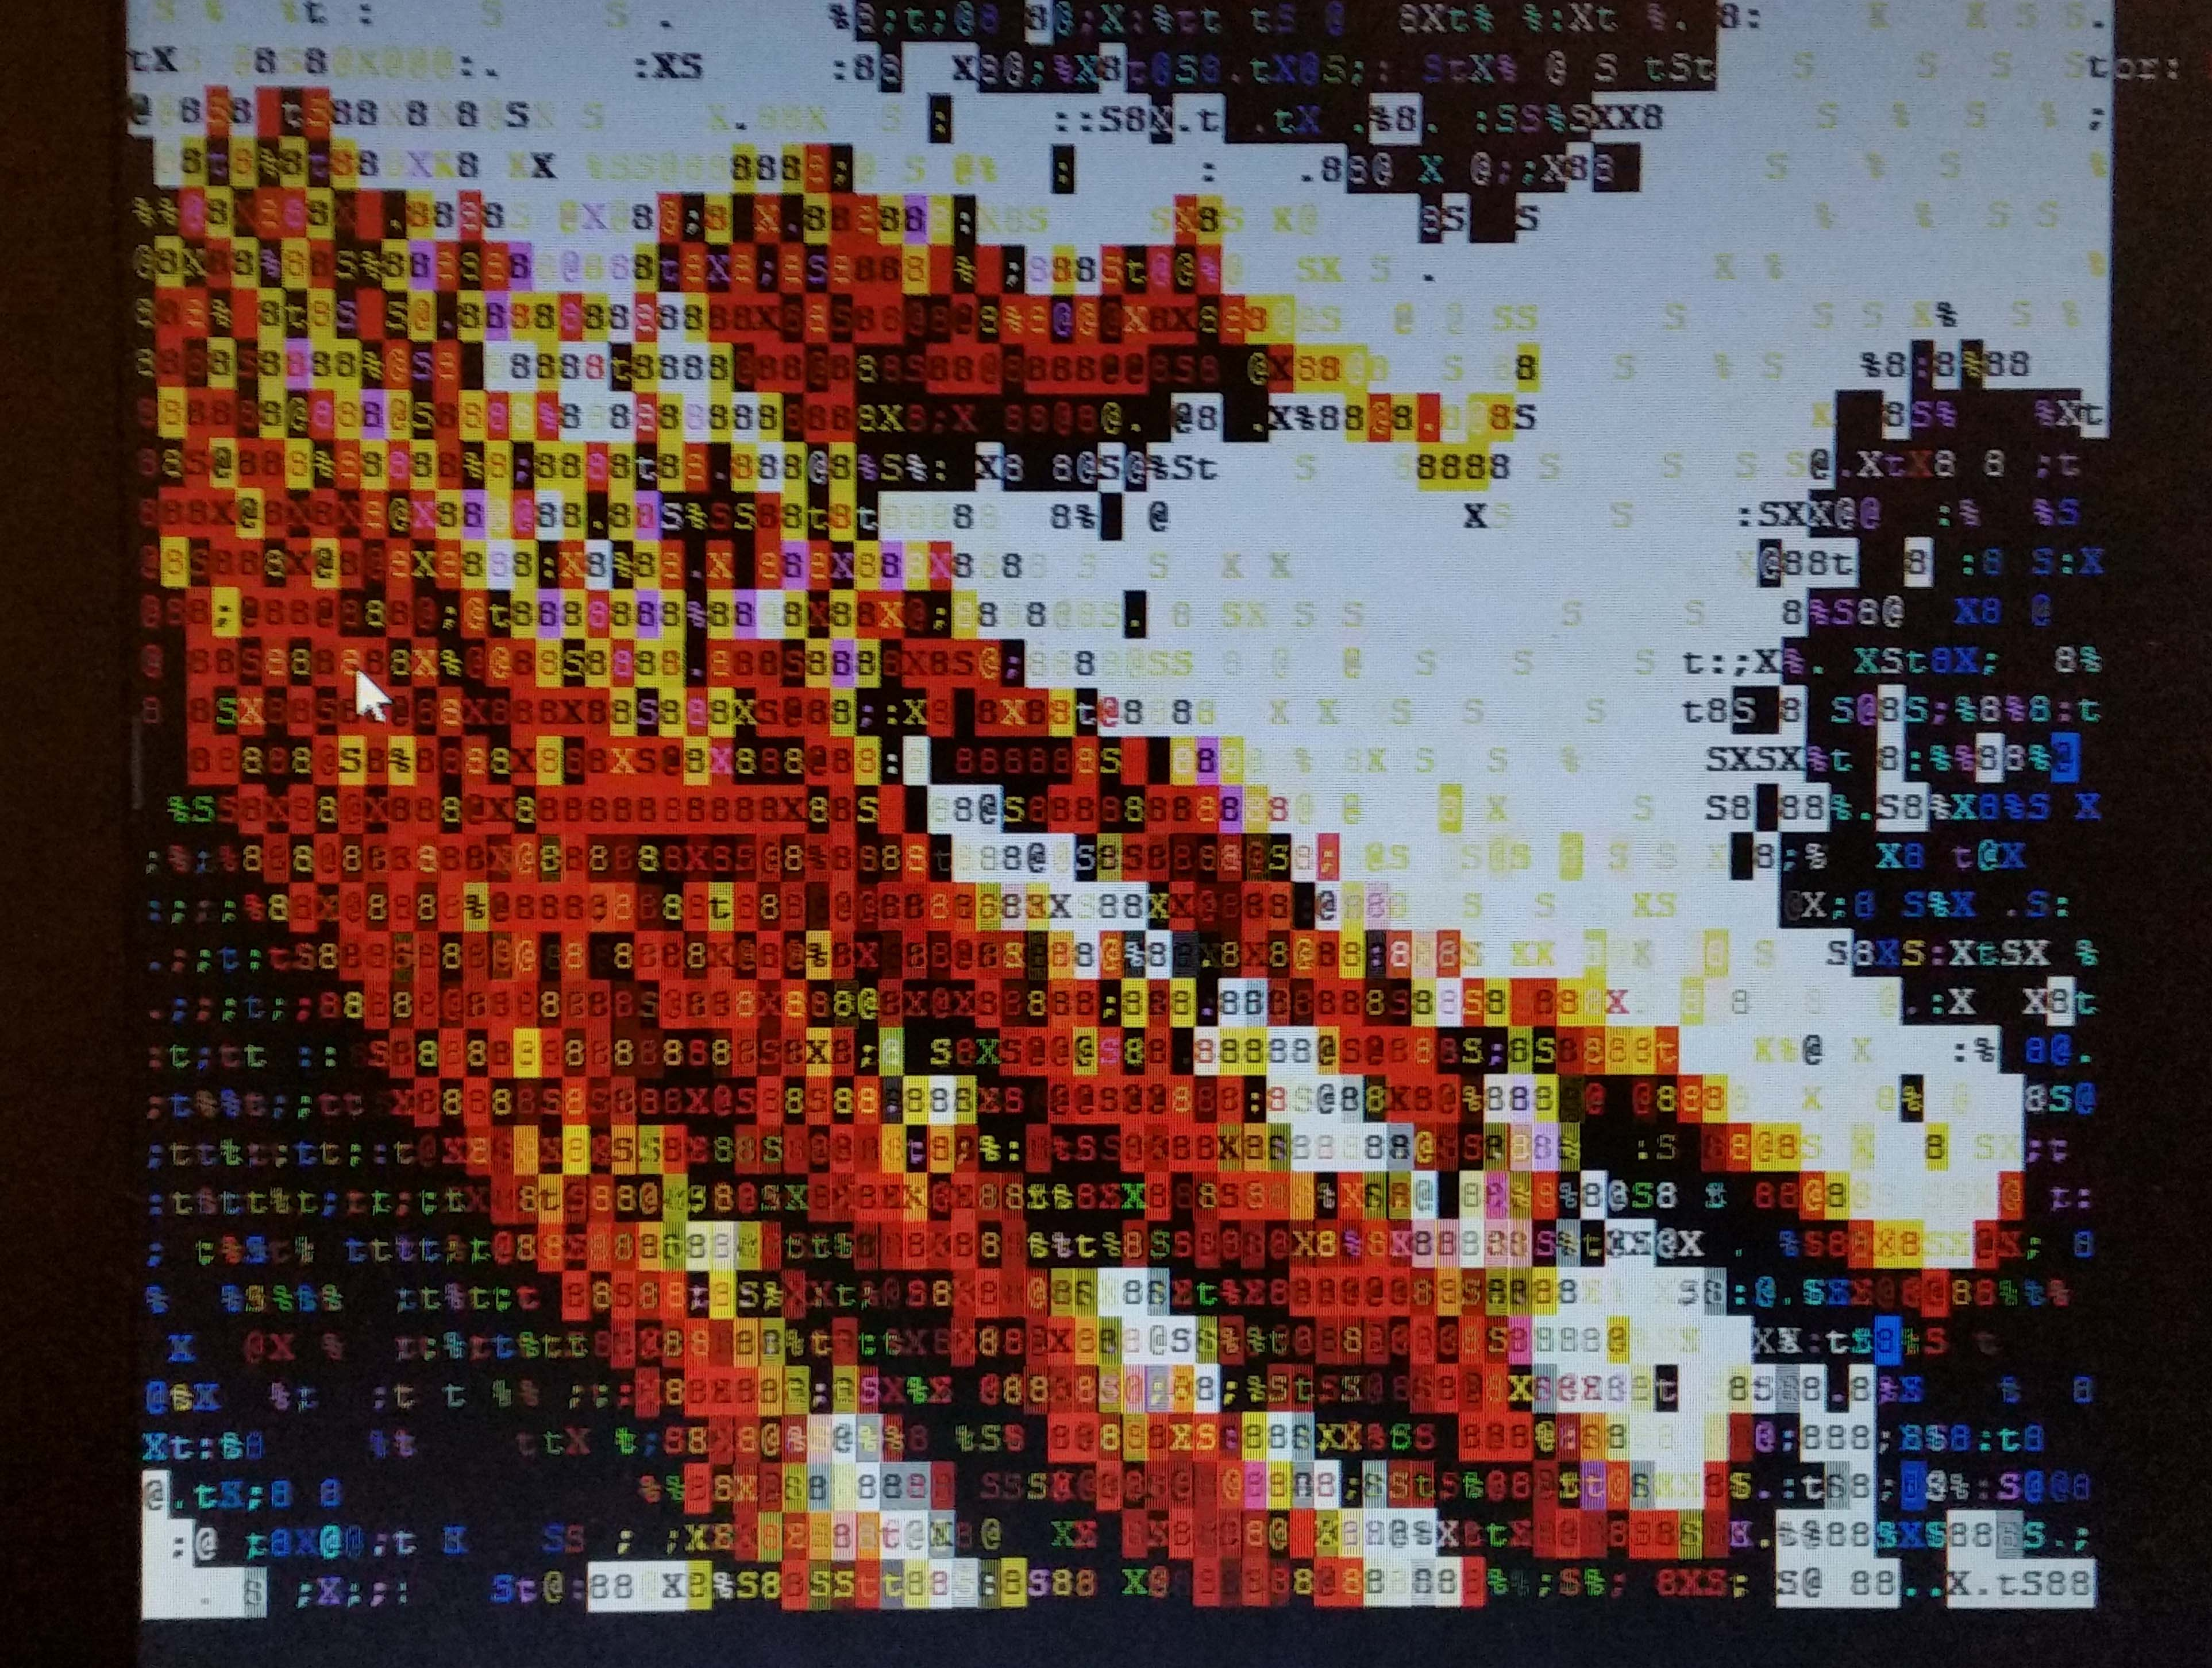
\includegraphics[width=5cm,%
                        keepaspectratio]{../UB1/images/8-8.jpg}%
                        \vfill}}}

\AtBeginDocument{%
        %
        % fancy setup
        %
        \fancyhf{}%
        \pagestyle{fancy}%
        \fancyheadoffset{1cm}%
        \fancyhead[L]{\small{\GetLecture}}%
        \fancyhead[R]{\small{Exercise \GetExercise}}%
        \fancyfoot[C]{\small{%
                \foreach \FirstName/\SecondName/\Email in \GetAutors%
                        { \FirstName \hspace{2mm}\SecondName \hspace{10mm}}}}
        \fancyfoot[R]{\small{\thepage}}%
        %
        \titleformat{\title}{\large\bfseries}{\thesection}{1em}{}%
        \titleformat{\section}{\large\bfseries}{\thesection}{1em}{}%
        \titleformat{\subsection}{\normalfont\fontsize{20}{15}\bfseries}{\thesubsection}{2em}{}%
        \titleformat{\subsubsection}{\normalfont\fontsize{18}{15}\bfseries}{\thesubsubsection}{2em}{}%
        %
        \AddToShipoutPicture*{\Logo{\GetLogo}}%
        \begin{titlepage}
        \flushright
        \rule{\linewidth}{0.5mm}\\ [0.5cm]
        {\bfseries \LARGE \GetLecture }\\
        {\bfseries \large Wintersemester 2015/2016 }\\ [2.0cm]
        {\bfseries \normalsize UNIVERSITÄT TÜBINGEN }\\ [3.0cm]

        \foreach \FirstName/\SecondName/\Email in \GetAutors
                {%
                \FirstName \hspace{2mm}%
                \SecondName%
                \hfill%
                \href{mailto:\Email}{\Email}%
                \\}
        \rule{\linewidth}{0.5mm}\\ [0.5cm]
        \flushleft
        {\bfseries \Huge Exercise \GetExercise }
\end{titlepage}
%
        \setcounter{section}{\GetExercise}
}

\newcommand{\xmark}{\ding{55}}


\SetLecture{Bildverarbeitung}
\SetExercise{1}
\AddAutor{Angel}{Rangel}{angel-eduardo.rangel-mendez@student.uni-tuebingen.de}
\AddAutor{Ido Freeman}{}{freeman@informatik.uni-tuebingen.de}
\AddAutor{Astrid Kreuzburg}{}{astrid.creuzburg@student.uni-tuebingen.de}
\SetLogo{mb}
\graphicspath{ {images/} }

%%Inicio documento
\begin{document} 
    \begin{enumerate}
         \item[Exercise 1:] Working with images
    \end{enumerate}
    \begin{enumerate}
        \item[(a)] {Write a function my loadImage that loads an image and display it (my showImage). Convert the image from uint8 to oating point representation (command double). Values should be in between 0 and 1. Use the functions image or imagesc.}
    \end{enumerate}
        \\ \ \\
        \\ \raggedright{ my loadImage:
        \\  img \ = \ double(imread(filename))/255;
        \\ \ \\ img is a 3-dimensional MxNx3 matrix, the elements in img(:,:,1) are interpreted as red  intensities, in img(:,:,2) as green intensities, and in img(:,:,3) as blue intensities.
        \\ \ \\ my showImage:
        \\ $ imagesc(img) $ }
        \\ \ \\ \ \\
    	\centering
        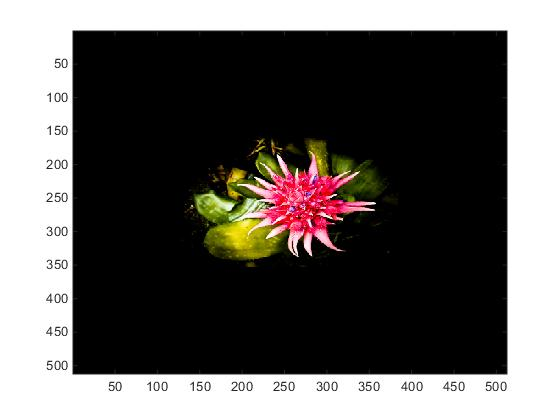
\includegraphics[scale=0.7]{images/SolutionFirstPart.jpg} 
\pagebreak
    \begin{enumerate}        
        \item[(b)] {Write two functions my RGBSplit and my plotRGBSplit that split the R, G and B channels of an image and display them separately. The plots should all be included in a single figure (use subplot). Each channel should be plotted in its primary color.}
    \end{enumerate}
        \raggedright{
        \\ my RGBSplit:
        \\ split the RGB channels:
        \\ imgR = imgRGB(:,:,1);
        \\ imgG = imgRGB(:,:,2);
        \\ imgB = imgRGB(:,:,3);
        \\ \ \\
        \\ my_plotRGBSplit:
        \\ Roff = struct('img', imgR, 'x', height0, 'y', width0);
        \\ Goff = struct('img', imgG, 'x', height1, 'y', width1);
        \\ Boff = struct('img', imgB, 'x', height2, 'y', width2);
        \\ \ \\
        \\ Icol = imgRGB;
        \\ \% figure layout
        \\ ax(1) = subplot(2,2,1);
        \\ Roff = mergeChannels(imgR, black, black);
        \\ im(1) = imshow(Roff);
        \\ title({'Red Channel'});
        \\ \ \\
        \\ ax(2) = subplot(2,2,2);
        \\ Goff = mergeChannels(black, imgG, black);
        \\ im(2) = imshow(Goff);
        \\ title({'Green Channel'});
        \\ \ \\
        \\ ax(3) = subplot(2,2,3);
        \\ Boff = mergeChannels(black, black, imgB);
        \\ im(3) = imshow(Boff);
        \\ title({'Blue Channel'});
        \\ \ \\
        \\ ax(4) = subplot(2,2,4);
        \\ im(4) = imshow(Icol);
        \\ title({'Original'});
        \\ end
        \\ \%funtion to merged
        \\ function merged = mergeChannels(a, b, c)
        \\    merged = cat(3, cat(3, a, b), c);
        \\ end
        \\ 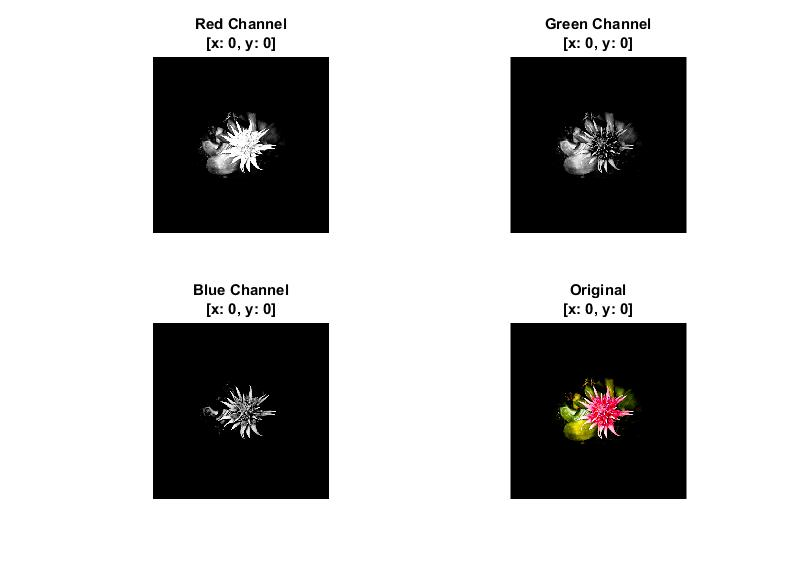
\includegraphics[scale=0.75]{images/SolutionSecPart.jpg} 
        }
\pagebreak
    \begin{enumerate}        
        \item[(c)] Implement a gamma correction for images (my gammaCorrection).
        \\
    \end{enumerate}
        \\
        Gamma Correction:
        \\ \ \\ imgGC = ((img) pow(1/GW));
        \\ \ \\
        \\ GW = 2.2; 
        \\ \     \\
        My showImage:
        \\ \ \\ imagesc(img)
        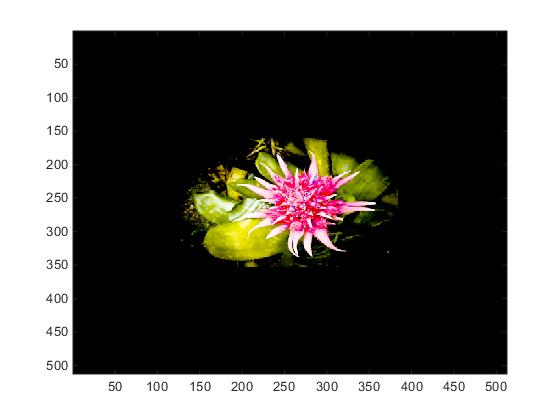
\includegraphics[scale=0.45]{images/SolutionFourth2Part.jpg}
        \\ GW = 0.8; \\
        \centering{
        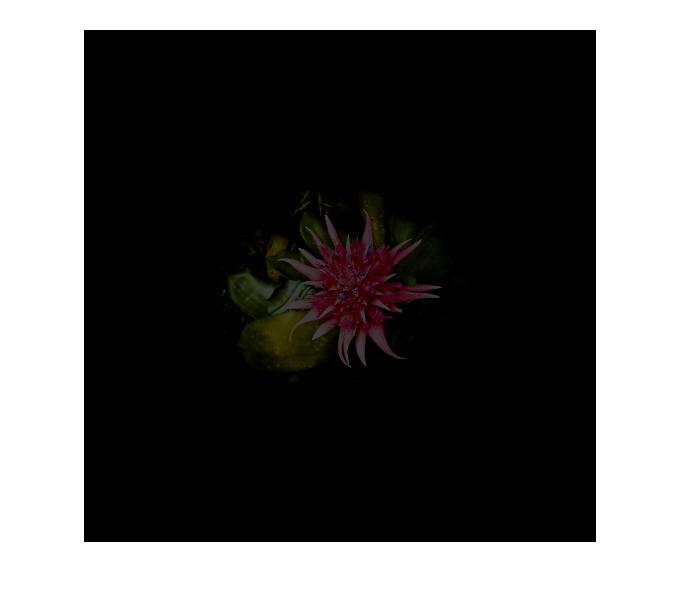
\includegraphics[scale=0.4]{images/SolutionFourthPart.jpg}
        } \\ 
\pagebreak
    \begin{enumerate}        
        \item[(d)] {Write a function my RGB2Gray that converts an image to grayscale. Apply your gamma correction before converting the image to grayscale.}
    \end{enumerate}        
        \\
        \\ \raggedright{ my RGB2Gray:
        \\\\ imgGC = my_gammaCorrection(img);
        \\ imgGray = zeros(size(img));
        \\
        \\ \% von Wikipedia
        \\ gray = 0.2126 .* imgGC(:,:,1) + 0.7152.*imgGC(:,:,2) + 0.0722.*imgGC(:,:,3);
        \\ for i=1:3
        \\ \ \ \ imgGray(:,:,i) = gray;
        \\ end
        \\\\ }
        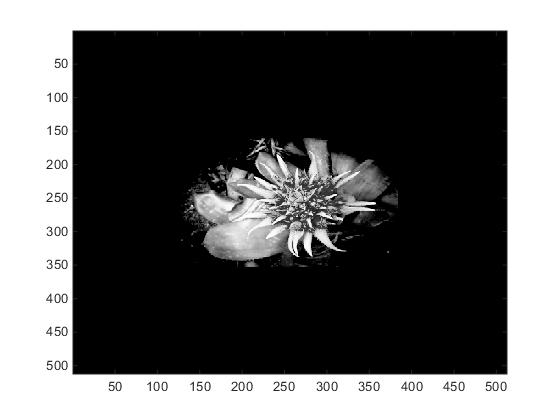
\includegraphics[scale=0.4]{images/SolutionImagD.jpg}
        \\ 
\pagebreak
    \begin{enumerate}
         \item[Exercise 2:] Histograms
    \end{enumerate}
    \\\\
    \begin{enumerate}        
        \item[(a)] {Create Histograms [2 points]: Implement a function "my hist" which computes the grayscale histogram of an image. Implement a plotting function for your histogram (my plotHist).
            Double-check your result using the Matlab functions hist or histc. What can be read out of the histogram  in general as well as for the given image?}
    \end{enumerate}
    \\\\
    \raggedright{
    \textbf{my hist:}
    \\ \ \\
    imgGray = uint8(imgGray*255);
    \\ [f,c]=size(imgGray);
    \\
    \\ for i=1:256
    \\ \ \ \ \ \ h(i) = 0;
    \\ end
    \\
    \\ for i=1:f
       \\ \ \ \ \ \ for j=1:c
           \\ \ \ \ \ \ \ \ \ \ \ k = imgGray(i,j);
           \\ \ \ \ \ \ \ \ \ \ \ h(k+1) = h(k+1)+1;
       \\ \ \ \ \ \ end
    \\ end
    \\ \ \\
    \\ hist = h;}
    \\ \ \\
    \textbf{my plotHist:}
    \\ \ \\
    figure;
    \\ plot(0:255, hist);
    \\ \ \\
    \centering{
    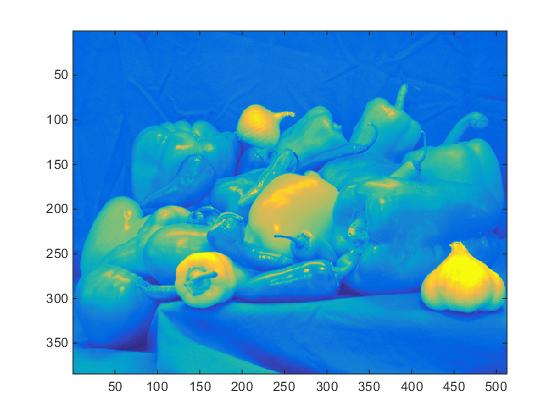
\includegraphics[scale=0.4]{images/2a1.jpg}
    \\ \ 
    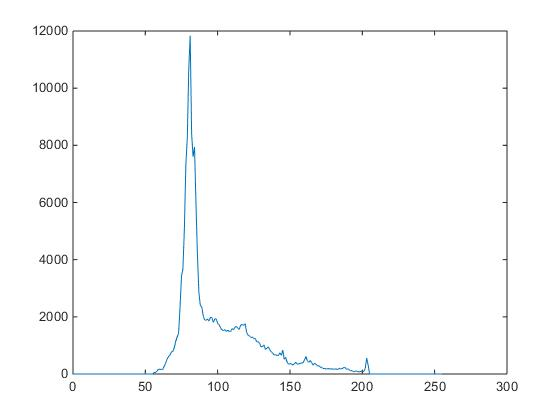
\includegraphics[scale=0.4]{images/2a2.jpg}
    \\ \ 
    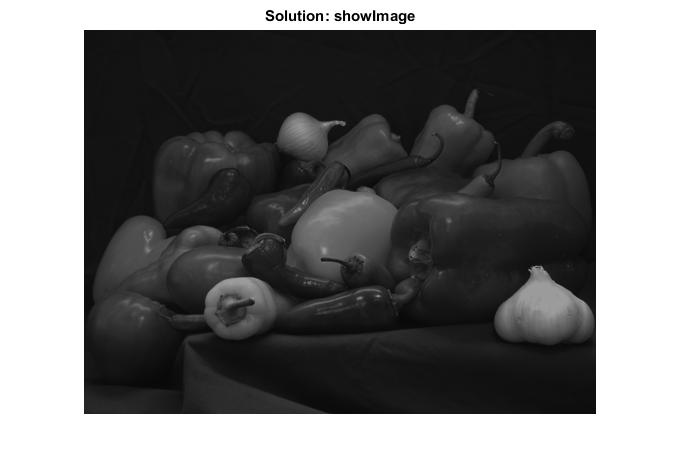
\includegraphics[scale=0.4]{images/2a3.jpg}
    \\ \ 
    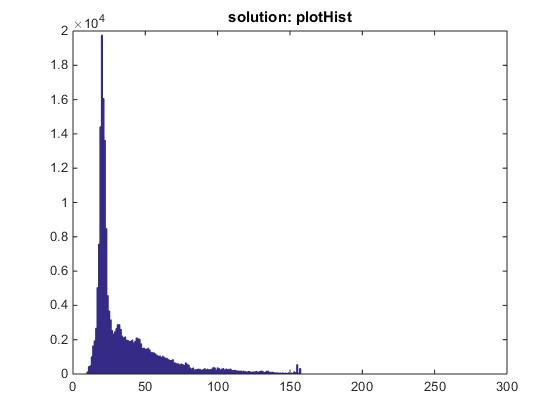
\includegraphics[scale=0.4]{images/2a4.jpg}
    }\\ \ 
    What can be read out of the histogram { in general as well as for the given image? TODO \pagebreak
    \begin{enumerate}        
        \item[(b)] {Contrast stretching [1 point]: Implement a function my maxContrast that maximizes the contrast of an image.}
    \end{enumerate}
    \\ \ \\
    
\end{document}